\chapter{Conceitos Gerais de IoT}
\label{chapter:coneceitos}

No capítulo \ref{chapter:intro}, foram vistos as bases para se implementar um projeto de IoT. A área começou a receber fortes investimentos e atenção por volta de 2009 e desde então foram feitas consideráveis implementações utilizando tecnologias e protocolos diferentes. Neste capítulo serão apresentados algumas dessas variantes, para fins de comparação e respaldo para importância e objetivo deste projeto.

\section{As Camadas da IoT}
\label{section:camadas_iot}

Uma rede IoT pode ser divida em camadas que exercem funções específicas no transporte de dados, de uma forma semelhante a redes de computadores, a camada acima não precisa saber como a inferior funciona, formando uma estrutura de pilha como na figura \ref{fig:1.2.0/camadas_iot}.

\begin{figure}[h!]
\centering
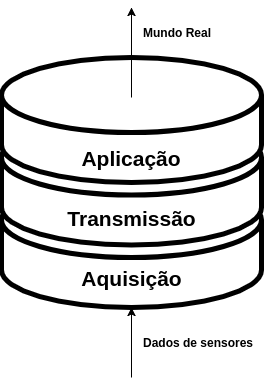
\includegraphics[width=5cm]{./02_Capitulos/02_Cap1/figures/iot_stack}
\caption{As três camadas do IoT, dos sensores ao mundo real}
\label{fig:1.2.0/camadas_iot}
\end{figure}

A primeira camada é a de aquisição de dados, que lida com o mundo físico e captura estes dados através de sensores e conversores A/D, também realiza o processamento para entregar em um formato adequado para transmissão e inteligível do outro lado, dependo da aplicação. A segunda camada é a camada de transmissão, na qual estão, efetivamente, as camadas de rede embutidas. Como o nome já denuncia, ela lida com os aspectos de rede e comunicação para que o dados cheguem seus destinos. E por último temos a camada de aplicação, a mais abrangente e que envolve maior poder computacional. Ela recebe os dados e lida com os processos de aplicação destes dados, seja análise, visualização, armazenamento ou a estruturação dos mesmos.

\subsection{Aquisição}
\label{subsection:aquisicao}

A etapa de aquisição está inserida diretamente no contexto de dados físicos, geralmente são hardwares menos complexos, focados em processamento de dados e entrada e saída com conversão analógico-digital. Se comunicam com sensores ou centrais de controle lógico. São responsáveis por:

\begin{itemize}
	\item Receber dados de sensores;
	\item Conversão A/D;
	\item Processamento de valores;
	\item Envio de dados em tempo real;
\end{itemize} 

Para atender essas tarefas, não é necessário grande poder de processamento, microcontroladores ou microprocessadores são capazes de atender aos requisitos necessários para uma grande gama de variáveis físicas, se acompanhados de módulos de rede e portas I/O, assim como a implementação do software. Serão vistos dois exemplos desses dispositivos, que utilizam tanto MCU  e outro um Consoles com Sistemas Operacionais leves.
 

\subsection{Transmissão}
\label{subsection:transmicao}

Esta camada é o coração do IoT. A transmissão define quais dispositivos eletrônicos e suas especificação técnicas. Também define como os softwares da camada de aplicação e aquisição devem ser implementados baseado na estrutura da pilha de rede que será usada para transmitir.

Na próxima seção, a camada de rede e suas formas de implementação serão detalhadas. É importante que esta camada seja definida da melhor forma a atender sua aplicação, alguns aspectos relevantes nesse sentido são:: 
\begin{itemize}
\item Quantidade de dados transmitido;
\item Número de acessos; 
\item Distância entre dispositivos;
\item Segurança;
\end{itemize}

\subsection{Aplicação}
\label{subsection:aplicacao}

A camada de aplicação encabeça a pilha do IoT. É ela que de fato trata os dados. Ela disponibiliza os dados para o mundo real, podendo exercer múltiplas funções simultâneas incluindo:

\begin{itemize}
\item Armazenamento e Análise; Através de Bancos de Dados e Aplicações;
\item Visualização; Aplicações Web, disponibilizando gráficos e tabelas de dados;
\item Inteligência e aprendizado; Machine Learning e Estatística para decisões e classificação;
\item Serviços e servidores; Aplicações em nuvem fornecendo microserviços em aplicações Web;
\end{itemize}

Nesta camada estão presentes as pontas apontados pela camada de aquisição, assim como os servidores que gerenciam os clientes (geralmente implementados na camada de aquisição) e serviços e configurações oferecidos pelo sistema em si.

\section{Redes de Computadores}
\label{section:camadas_de_rede}

Como visto anteriormente, a camada de transmissão basicamente define a infraestrutura do sistema. Ela é construída baseada em como a rede é implementada. Redes de computadores são complexas com diferentes aspectos a se preocupar. Dividir em camadas permite modularizar a implementação da rede, de modo que cada camada tenha uma tarefa na estrutura de comunicação dos aspectos físicos ao software. Como uma camada  não precisa saber os detalhes e especificações da camada logo abaixo. Existem diversas formas de implementação de camadas, mas todas se baseiam em um modelo de referência, o modelo OSI \cite{Zimmermann:1988:ORM:59309.59310}.


\begin{figure}[h!]
\centering
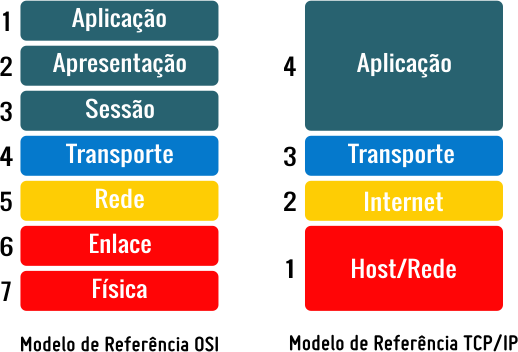
\includegraphics[width=8cm]{./02_Capitulos/02_Cap1/figures/modelo_osi_tcpip}
\caption{Diferenças entre OSI e TCP/IP em suas camadas}
\label{fig:1.2.0/modelo_osi_tcpip}
\end{figure}

Baseado no modelo OSI, temos o modelo TCP/IP \cite{TCPIP}, visualizado na \ref{fig:1.2.0/modelo_osi_tcpip} e utilizado na internet e base para protocolos de aplicação muito utilizados como HTTP, WebSocket e MQTT. Em ambos cada camada exerce uma tarefa com seu respectivo protocolo. O protocolo define regras e convenções para a comunicação entre dispositivos em rede. A \ref{table:1.2.0} resume os detalhes de cada camada.

\begin{table}[h]
\centering
\caption{As camadas e e suas funções}
\begin{tabular}{|l|l|}
\hline
\multicolumn{1}{|c|}{CAMADA} & \multicolumn{1}{c|}{DETALHES}                                                  \\ \hline
7 - Aplicação                & Define instruções específicas da aplicação          						    \\ \hline
6 - Apresentação             & Formatação dos dados, conversão dos dados                     					\\ \hline
5 - Sessão                   & Negociação e conexão com outros nós.                                \\ \hline
4 - Transporte               & Oferece métodos para a entrega de ponta-a-ponta                        			\\ \hline
3 - Rede                     & Roteamento e endereçamento de pacotes em uma ou várias redes                                 \\ \hline
2 - Enlace                   & Detecção de erros, transmissão e recepção de quadros e controle de fluxo.                                                          \\ \hline
1 - Física                   & Aspectos físicos da transmissão \\ \hline
\end{tabular}
\label{table:1.2.0}
\end{table}


O projeto lidará com aspectos e protocolos da camada de Aplicação. Apesar de diferentes tecnologias utilizarem diferentes camadas abaixo, serão especificas características de protocolos construídos sobre o TCP/IP, por seu uso na internet e redes industriais, e que sejam eficientes em trocas de mensagens em tempo real.

\section{Tecnologias em IoT}
\label{section:tecnologias_iot}

As primeiras aplicações de IoT foram em laboratórios com RFID \cite{Rampim:iot}, junto com códigos bidimensionais (como o QR Code), para aplicações de identificação de objetos, é uma das soluções mais populares e de baixo custo de IoT utilizando Rádio frequência.

Redes que utilizam bandas restritas visando baixo consumo e distância de transmissão, são utiizadas em redes IoT de celulares e irão se tornar opções dominantes de conectivdade com o advento do 5G. As NB-IoT concentram-se especificamente na cobertura interna, baixo custo, longa duração da bateria e alta densidade de conexão. As mensagens de IoT são geralmente curtas, dados telemétricos, status etc. Já se encontram implementadas algumas redes como SigFox \cite{Sigfox} e LoRa \cite{LoRa}. 

As novas gerações de Bluetooth consomem muito menos energia, o que tornaram a tecnologia viável para aplicações IoT. Geralmente, módulos Bluetooth são utilizados como beacons \cite{Endeavor:Beacons}. Pontos espalhados por uma região, no qual podem se comunicar com os módulos de dispositivos mobile ao se aproximar, oferecendo links para conteúdo e exclusividades.

As tecnologias mais comuns de se encontrar em aplicações IoT, os protocolos construídos com base no TCP/IP são vastamente utilizados e possuem uma rede mundialmente distribuída, o que facilita o uso. Pode-se implementar uma gama de protocolos de aplicações, alguns mais eficientes que outros.

O protocolo mais simples seria o HTTP, altamente usado na internet, porém não é eficiente no consumo de energia por abrir uma conexão a cada envio de dados. Para minimizar estas desvantagens, foi desenvolvido o CoAP (Constrained Application Protocol) \cite{coap} protocolo nos mesmos moldes do HTTP com arquitetura REST (Representational State Transfer), que define as regras para criação de uma serviços Web, garantindo interoperabilidade entre sistemas e a Internet. Entretanto o CoAP é mais simples, mais leve, com baixo overhead e utilizado em redes locais.

Mas os mais utilizados em aplicações são sem dúvidas os protocolos que mantém conexão aberta, em especial Websocket e MQTT, sendo o primeiro mais utilizado para chats e mensagens, enquanto o segundo domina o mundo do M2M e Telemetria.


\section{Arquiteturas de Protocolos}
\label{section:arquitetura_protocolo}


%%% MQTT , Websocket e HTTP %%%
Existem protocolos de aplicação que podem ser facilmente mapeados por esse tipo de interface. Alguns já são cosntruídos no modelo Publish/Subscribe, outros em modelos parecidos. Para critérios de comparação, apresentam-se dois protocolos de aplicação, MQTT e WebSockets \cite{websocket}. O protocolo MQTT, no qual será implementado nesse projeto, foi moldado no padrão citado, enquanto o WebSockets é orientado a eventos. Ambos enviam mensagens em tempo real através de um servidor que controla o fluxo de mensagens da aplicação.

\subsection{MQTT X HTTP}
\label{subsection:mqttxhttp}

Na questão de desempenho, estes protocolos se mostram mais eficientes dentre os construídos sobre TCP/IP, comparado, por exemplo, com o HTTP, protocolo de rede mais recorrente em redes locais e na internet. Como mostrado em \cite{Tetsuya-Sasaki} e \cite{Naik}, HTTP, por sua natureza de abrir e fechar conexão a cada requisição de dados e seu cabeçalho ilustrado na \ref{fig:3.2.0/http-flow}, requer mais banda e consome mais energia que protocolos leves e de conexão persistente como o MQTT. O que faz sua escolha remota para a aplicação deste projeto.

\begin{figure}[h]
\centering
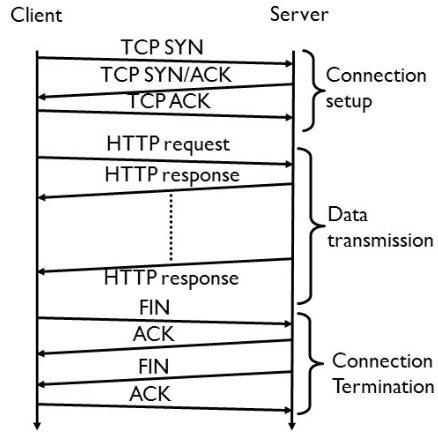
\includegraphics[width=8cm]{./02_Capitulos/02_Cap3/figures/http-flow}
\caption{Fluxo de conexão do HTTP}
\label{fig:3.2.0/http-flow}
\end{figure}

Já o MQTT é um protocolo de cabeçalhos menores, conexão persistente e menos passos para o envio de mensagem, como visto na \ref{fig:3.2.0/mqtt-flow}, por ser um protocolo feito com o objetivo de reduzir a latência, levando vantagem para a transmissão contínua de dados, em relação ao HTTP.

\begin{figure}[h]
\centering
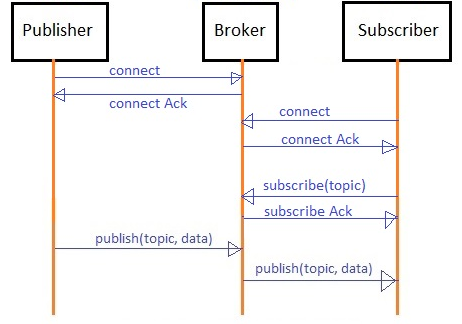
\includegraphics[width=8cm]{./02_Capitulos/02_Cap3/figures/mqtt-flow}
\caption{Fluxo da conexão do MQTT}
\label{fig:3.2.0/mqtt-flow}
\end{figure}

Abaixo na \ref{tabela:mqttxhttp} encontra-se o resumo comparativo entre os protocolos MQTT e HTTP:

\begin{table}[h!]
\caption{Comparativo MQTT X HTTP}
\resizebox{\textwidth}{!}{%
\begin{tabular}{|l|l|l|}
\hline
\textbf{Característica-Protocolo}     & \textbf{MQTT}                           & \textbf{HTTP}         \\ \hline
\textbf{Arquitetura}                  & Publish/Subscribe                       & Request/Response      \\ \hline
\textbf{Complexidade}                 & simples                                 & complexa              \\ \hline
\textbf{Segurança}                    & TSL/SSL                                 & TSL/SSL               \\ \hline
\textbf{Camada de Transporte}         & TCP                                     & TCP ou UDP            \\ \hline
\textbf{Tamanho/Formato de Mensagens} & curtas, binário com cabeçalho de 2Bytes & Grande, Formato ASCII \\ \hline
\textbf{Porta Padrão}                 & 1883                                    & 80 ou 8080            \\ \hline
\textbf{Distribuição de dados}        & 1 um para 0/1/N                         & um para um            \\ \hline
\end{tabular}%
}
\label{tabela:mqttxhttp}
\end{table}



\subsection{MQTT}
\label{subsection:mqtt}

O protocolo MQTT foi utilizado escolhido por ser leve e ideal para aplicações em tempo real com vários dispositivos simultaneamente. É um protocolo no padrão Publish/Subscribe  ideal para definir a função de cada dispositivo seja enviando dados (Publish) ou recebendo estes (Subscribe).

Para gerenciar os clients (responsáveis pela implementação da comunicação MQTT) em cada dispositivo é necessário um servidor chamado Broker. Este foi implementado com o Mosquitto \cite{mosquitto}, um broker open source e leve capaz de ser instalado localmente e no servidor do laboratório para testes remotos.

\section{Publishers e Subscribers}
\label{section:publishers_subscribers}

Para enviar e receber dados de uma forma a atender os requisitos da seção \ref{section:interface}, foi utilizado um padrão de comunicação recorrente em aplicações contemporâneas, o padrão Publish/Subscriber \cite{amazon:pub-sub}.

O padrão Publish/Subscribe permite que as mensagens sejam transmitidas assíncronas e para vários dispositivos simultaneamente. Para transmitir uma mensagem, um client pode simplesmente enviar uma mensagem para o tópico que os envia imediatamente para todos os subscribers. Todos os componentes que se inscreverem no tópico receberão todas as mensagens transmitidas, a menos que uma política de filtragem de mensagens seja definida pelo assinante.

\begin{figure}[h!]
\centering
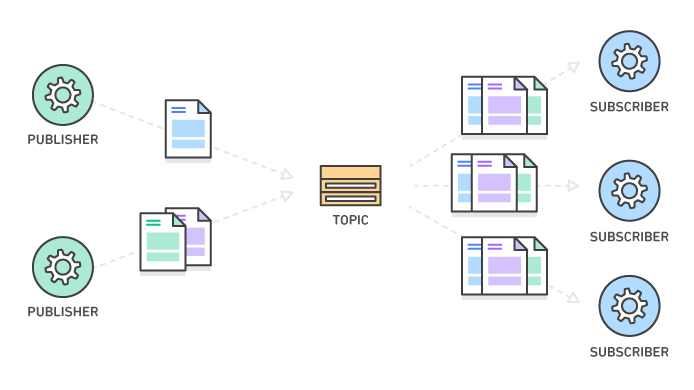
\includegraphics[width=12cm]{./02_Capitulos/02_Cap3/figures/aws_pub_sub}
\caption{O padrão Publish/Subscribe. Retirado de \cite{amazon:pub-sub}}
\label{fig:3.2.0/aws_pub_sub}
\end{figure}

Qualquer mensagem publicada em um tópico é imediatamente recebida por todos os subscribers do tópico. As mensagens de podem ser usadas para arquiteturas orientadas a eventos ou para desacoplar aplicativos, aumentando  o desempenho, a confiabilidade e a escalabilidade. Com isso, foram criados duas funções possíveis para cada dispositivo dentro deste padrão, os Publishers e os Subscribers, sua comunicação é descrita em \ref{fig:3.2.0/pub_sub}.

\subsubsection{Broker}
\label{subsubsection:broker}

O Broker é o servidor do padrão Publish/Subscribe, ele efetivamente executa as ordens de publicação (publish) feita por algum cliente para os tópicos que outros clientes estão inscritos (subscribed), possui todas as listas de tópicos, é orientado a conexão e não persiste informações dos clientes, ou seja, em caso de queda de conexão, estes devem se inscrever novamente nos tópicos.

\textit{Nota: A arquitetura Broker não é exclusividade do MQTT, outros protocolos utilizam esse tipo de implementação em servidores.}


\begin{figure}[h]
\centering
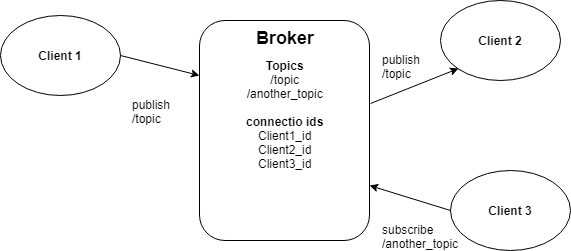
\includegraphics[width=12cm]{./02_Capitulos/02_Cap3/figures/broker_pub_sub}
\caption{Exemplo de gerênciamento de um broker}
\label{fig:3.2.0/broker_pub_sub}
\end{figure}

Na figura \ref{fig:3.2.0/broker_pub_sub}, o Broker armazena os tópicos e os ids de conexão dos clientes, 2 estava inscrito para ouvir as mensagens do tópico \textit{topic}, enquanto 3 enviava uma ordem de inscrição em \textit{another\_topic}, 1 envia ordem de publicação para \textit{topic}.


\subsubsection{Tipos de MQTT}
\label{subsubsection:tipos_mqtt}

%% Tipos de MQTT 
Com a evolução e o uso do protocolo, foram necessárias atualizações que contemplam funcionalidades que atendem  requisitos essenciais para aplicações da indústria. Como atender dispositivos que não usam a pilha TCP/IP e medidas de segurança (que serão melhor debatidas á frente). 

Existe uma gama de dispositivos que utilizam protocolos específicos, geralmente leves, para redes locais e leves para o transporte de dado, a exemplo do ZigBee \cite{zigbee}. Para isso foi criada uma versão do MQTT para atender estes tipos de protocolos, substituindo a base TCP/IP por outros protocolos destas camadas, mantendo a camada de aplicação e o padrão Publish/Subscribe.

Para resolver questões de segurança, foi criada uma variação do MQTT que adiciona camadas deste quesito ao protocolo de aplicação. Assim como o HTTPS o protocolo MQTTS é construído em cima do protocolo SSL/TLS (explicado em \ref{subsection:seguranca}), camada de segurança que também usa como base TCP/IP. Esta camada envolve o processo de encriptação dos cabeçalhos da aplicação e autenticação por passagem de certificados.

\section{Segurança de aplicações}
\label{section:seguranca}

%% SSL e outros tipos de encriptação de dados.
SSL \cite{ssl} (Secure Sockets Layer) é a tecnologia de segurança padrão para estabelecer um link criptografado entre um servidor da Web e um cliente. Um certificado SSL em seu servidor e um navegador se conecta a ele, a presença do certificado SSL aciona o protocolo SSL (ou TLS), que criptografa as informações enviadas entre o servidor e cliente.

O SSL opera diretamente no topo do protocolo de controle de transmissão (TCP), além de permitir que camadas de protocolo de aplicaçãoes sejam construídas por cima, agora com sob uma camada de segurança. Portanto, sob a camada SSL, as outras camadas de protocolo podem funcionar normalmente, como o HTTP e o MQTT.

Com um certificado SSL, todos os invasores poderão saber qual IP e porta e quantos dados estão sendo enviados. Eles podem terminar a conexão, mas tanto o servidor quanto o usuário poderão dizer que isso foi feito por terceiros. No entanto, eles não serão capazes de interceptar qualquer informação, o que a torna essencialmente um passo ineficaz. O invasor pode descobrir qual nome de host,mas como a conexão é criptografada, as informações importantes permanecem seguras.

Para poder criar uma conexão é requisitado um Certificado SSL. Quando você optar por ativar o SSL em seu servidor da Web, será solicitado que você responda a várias perguntas sobre a identidade do seu site e da sua empresa. Seu servidor da Web cria duas chaves criptográficas - uma chave privada e uma chave pública.

A chave pública não precisa ser secreta e é colocada em uma solicitação de assinatura de certificado (CSR) - um arquivo de dados que também contém seus detalhes, então deve-se enviar o CSR. Durante o processo de solicitação do Certificado SSL, a Autoridade de Certificação validará seus detalhes e emitirá um Certificado SSL contendo seus detalhes e permitindo que você use SSL.

Além do SSL existem outras formas de segurança. A maioria envolve encriptação. Como o uso de algoritmos de hash para encriptar as mensagens enviadas, ficando a cargo da aplicação desencriptar.

A Interface aqui construída é transparente ao SSL, ou seja, pode ser implementada em cima ou não deste protocolo, os exemplos são feitos sem esta camada, porém basta criar ou adquirir um certificado em uma autoridade de certificação e gerar as chaves. As APIs usadas contemplam da opção de usarem clients SSL.


\section{Persistência de dados}
\label{section:persistencia}

%% Bancos de dados
Os dados adquiridos pela plataforma e suas camadas, são armazenados em memórias e enviados. Memórias voláteis que podem facilmente perder dados com quedas de energia o reaproveitamento do sobre-inscrição do próprio gerenciamento do sistemas, para garantir que os dados não sejam perdidos, é necessário que o sistema possua persistência, uma forma de memória não-volátil que armazene os dados sem energia.

Essa persistência é implementada com Banco de Dados, estruturas que organizam o armazenamento de dados persistentes em arquivos. Um Banco de dados é uma basicamente uma aplicação, um serviço do sistema que recebe requisições de rede e escreve ou lê dados em um arquivo. Existem inúmeras formas de implementação e protocolos de comunicação para Bancos de Dados. Porém todos eles seguem abstrações em comum.

Um banco é composto por duas ferramentas. O Motor e o Arquivo de dados. O motor é quem realiza as ações sobre o arquivo, é o sistema de gerenciamento. Recebe as requisições e aplica algoritmos de escrita de dados eficientes no arquivo para armazenar os dados em uma estrutura definida. Um Banco de dados pode possuir vários motores, cada um com algum algoritmo que varia a eficiência e o tempo de escrita e/ou leitura dependendo do dado recebido.

\begin{figure}[h!]
\centering
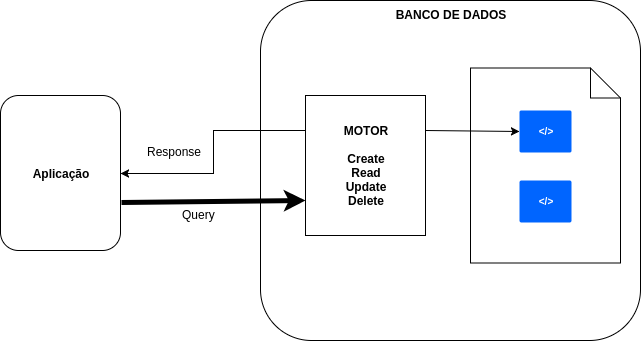
\includegraphics[width=12cm]{./02_Capitulos/02_Cap3/figures/Database_Arch}
\caption{A arquitetura de um banco de dados}
\label{fig:3.3.5/database_arch}
\end{figure}

O Arquivo é o documento onde os dados são armazenados, na estrutura definida. Possuem formatações de dados específicas de cada tipo de banco, seguindo uma abstração. O formato do armazenamento de dados, define e limita eficiência do motor, então e necessário a escolha adequada de algoritmo para uma maior eficiência da leitura do arquivo. Como em \ref{fig:3.3.5/database_arch} a aplicação envia uma solicitação de criação ou leitura ou atualização ou remoção (CRUD - Create, Read, Update, Delete) e o motor lida com os dados, armazenando-os em uma determinada estrutura no Arquivo.


 
\section{Bancos para Aplicações IoT}
\label{section:bancos_IoT}

Na área de Bancos de Dados (ou DBs), com escopo focado em IoT, há um porém. Para a estruturação de uma aplicação eficiente, não se deve usar qualquer tipo de banco. Devem-se escolher motores e estruturas de bancos adequadas para a aplicação. Não exite um critério definitivo que guia o desenvolvedor para melhor escolha. Mas algumas características de bancos de dados podem ser exploradas em aplicações IoT, formando um DB eficiente para tal.

Como pode ser observado em \cite{Damodaran}, uma aplicação eficiente de Bancos e IoT está ligada ao tempo de inserção de dados no banco,  o tempo total em que a aplicação leva para enviar, aplicar a busca de onde o dado deve ser inserido no documento e de fato armazenar, podem ser feitas várias inserções de pequenos pacotes de dados, dependendo do tamanho da mensagem. Esta característica está ligada ao motor do banco, que determina como o dado será armazenado, e quanto ele leva para escrever o dado no documento. A maioria dos dados são armazenados em estruturas B+Trees \cite{b-tree}, porém pode-se observar em \cite{Damodaran} que a estrutura LSM Tree \cite{O'Neal-Gawlick-Cheng} possui maior eficiência na escrita.


\begin{figure}[h!]
\centering
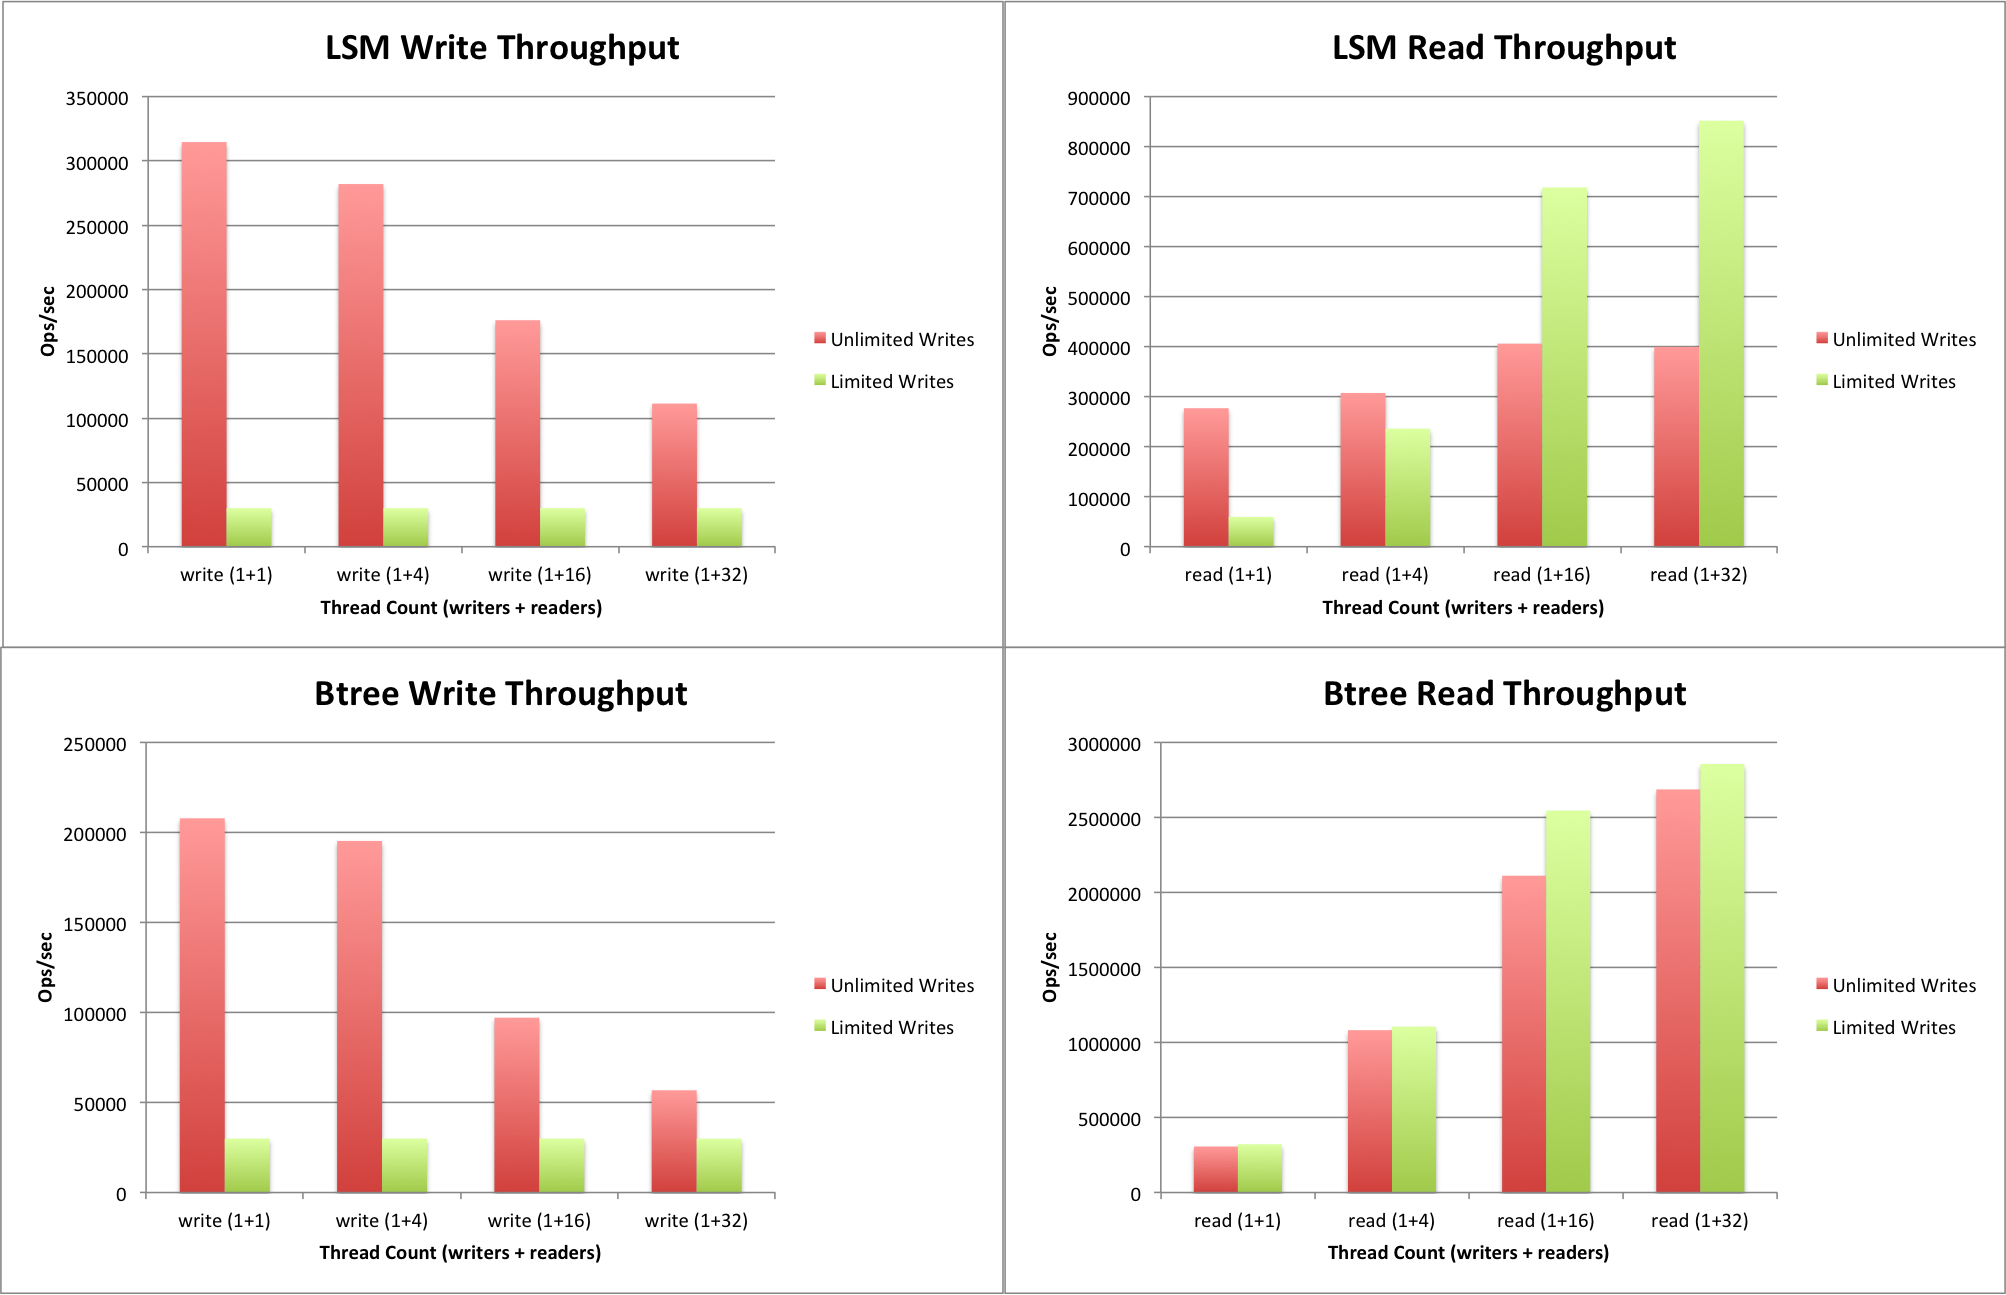
\includegraphics[width=14cm]{./02_Capitulos/02_Cap3/figures/LSM_btree}
\caption{Comparação de Escrita e Leitura entre LSM e B+, retirado de \cite{btrees-vs-lsmtrees}}
\label{fig:3.3.5/b-lsm}
\end{figure}

Comparando as duas estruturas, como mostrado em \ref{fig:3.3.5/b-lsm}, percebe-se que a estrutura LSM sustenta até 2x mais inserções da estrutura B+, hoje os Bancos de Dados modernos utilizam desta vantagem, devida a nova tendência de aplicações de coletar dados constantemente, o que leva a operação de escrita no banco ter mais importância e ocorrências que a leitura e explica a migração para a estrutura LSM.

Existem várias abstrações de Bancos de dados. Em \cite{Rautmare-Bhalerao} compara-se e conclui-se que o banco MongoDB, um banco NoSQL possui um tempo de resposta de inserção menor que o MySQL (bancos relacionais), porém o último é mais estável. De fato bancos NoSQL são, em geral, mais leves, possui uma flexibilidade maior para lidar e estruturar dados, o que fazem estes tipos de Banco mais favoráveis a aplicações de IoT. Porém outras estruturas como um banco divido em timescale mostram-se eficientes SQL ou não.

Outros aspectos podem contribuir para a eficiência de persistência de dados. Criar bancos locais diminuem a latência e a necessecidade de conexão, aumentando a capacidade de inserção de dados, além de ser uma forma de backup de dados. Um banco local, geralmente fica em uma plataforma como em \cite{Paethong-Sato-Namiki}, são bancos leves em aplicações de baixo consumo, devido a capacidade de processamento limitada. Seu papel é geralmente para armazenar os dados quando não há conexão, e quando esta é restabelecida os dados são enviados para um banco remoto com mais capacidade de processamento e aplicações. %% Falar sobre bancos locais.

Dentre os bancos estudados, alguns se destacam como o Cassandra, usado pela Netflix para coletar dados sobre o comportamento do usuário na plataforma ou o InfluxDB, um banco de arquitetura TimeScale, feito para aplicações em tempo real. Mas para esse projeto, foi utilizado o MongoDB \cite{mongodb}, um banco NoSQL, leve, de facil integração com as plataformas utilizadas e que posui implementações de motores que priorizam a eficiência na escrita de dados, como a LSM tree.




